\documentclass[border=4pt]{standalone}
\usepackage{tikz}
\begin{document}
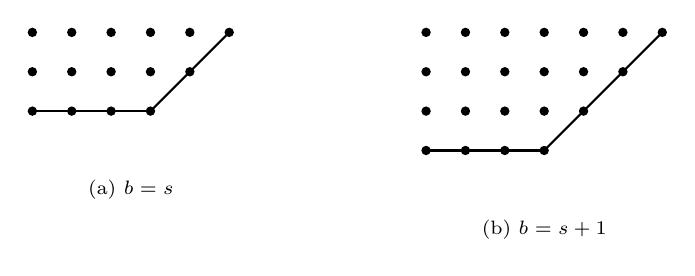
\begin{tikzpicture}[scale=0.5,dot/.style={circle,fill,inner sep=1.2pt}]
  % (a) b = s : partition 6+5+4+... base of 4? use rows 7,6,5,4 with base 4=s
  \begin{scope}
    \foreach \len [count=\r from 0] in {6,5,4} {
      \foreach \c in {1,...,\len} \node[dot] at (\c,-\r) {};
    }
    \draw[thick] (6,0) -- (4,-2);
    \draw[thick] (1,-2) -- (4,-2);
    \node at (3.5,-4) {\scriptsize (a) $b=s$};
  \end{scope}
  % (b) b = s+1
  \begin{scope}[xshift=10cm]
    \foreach \len [count=\r from 0] in {7,6,5,4} {
      \foreach \c in {1,...,\len} \node[dot] at (\c,-\r) {};
    }
    \draw[thick] (7,0) -- (4,-3);
    \draw[thick] (1,-3) -- (4,-3);
    \node at (4,-5) {\scriptsize (b) $b=s+1$};
  \end{scope}
\end{tikzpicture}
\end{document}
